\begin{frame}{Gradient Boosting -- method summary}

% \maketag{supervised} 
\maketag{regression} \maketag{classification}
\maketag[50]{(NON)PARAMETRIC}
\maketag{BLACK-BOX}
\maketag{FEATURE SELECTION}

\medskip

\highlight{General idea}

\begin{itemize}
  \item Create \textbf{ensemble} in \textbf{sequential}, stage-wise manner
  \begin{itemize}
    \item In each iteration, add new model component in risk-minimal fashion
    \item Final model: weighted sum of base learners (frequently, \textbf{CART})
  \end{itemize}
  \item Fit each base learner to current \textbf{point-wise residuals} 
  \\ $\Rightarrow$ one boosting iteration $\widehat{=}$ one approximate 
  \textbf{gradient step in function space}
\end{itemize}

\medskip

\highlight{Hypothesis space} ~~
$\Hspace = \left\{ \fx: \fx = \sum_{m = 1}^M \betam b(\xv, \thetam) \right\}$

\begin{minipage}{0.45\textwidth}
  \centering
  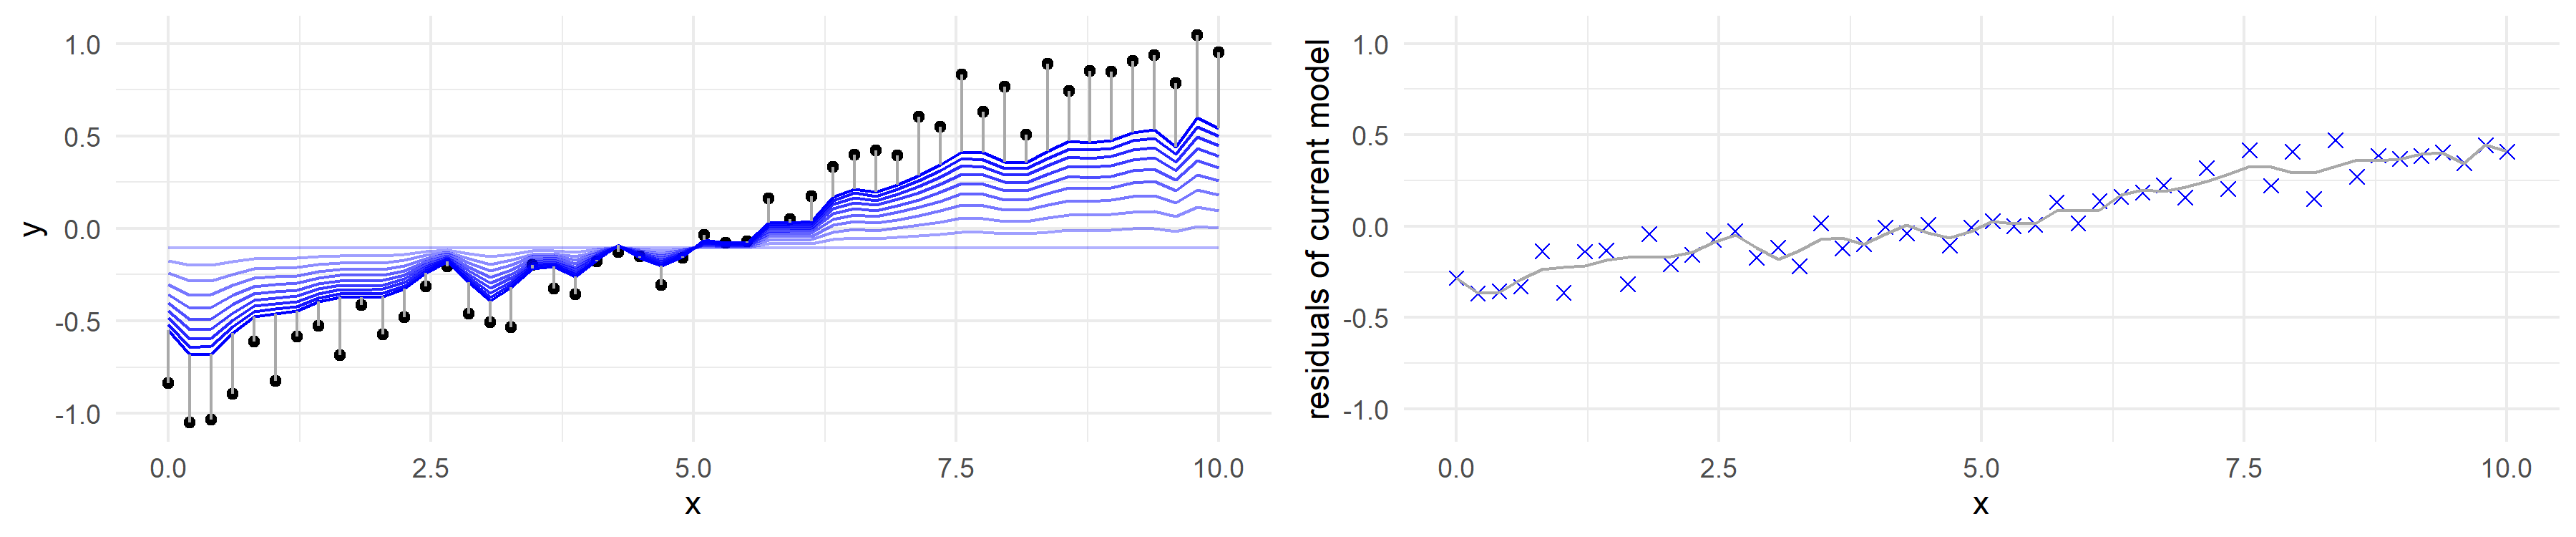
\includegraphics[width=\textwidth, trim=0 0 450 0, clip]{
  ../slides/boosting/figure/illustration_gaussian_huber_2_10} \\
  \tiny{Boosting prediction function with GAM base learners for univariate 
  regression problem after 10 iterations}
\end{minipage}%
\hfill
\begin{minipage}{0.45\textwidth}
  % FIGURE SOURCE: http://arogozhnikov.github.io/2016/06/24/gradient_boosting_explained.html
  % 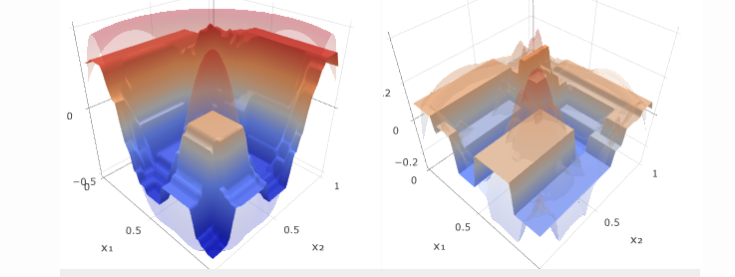
\includegraphics[width=\textwidth]{figure/gb-3d} \\
  \centering
  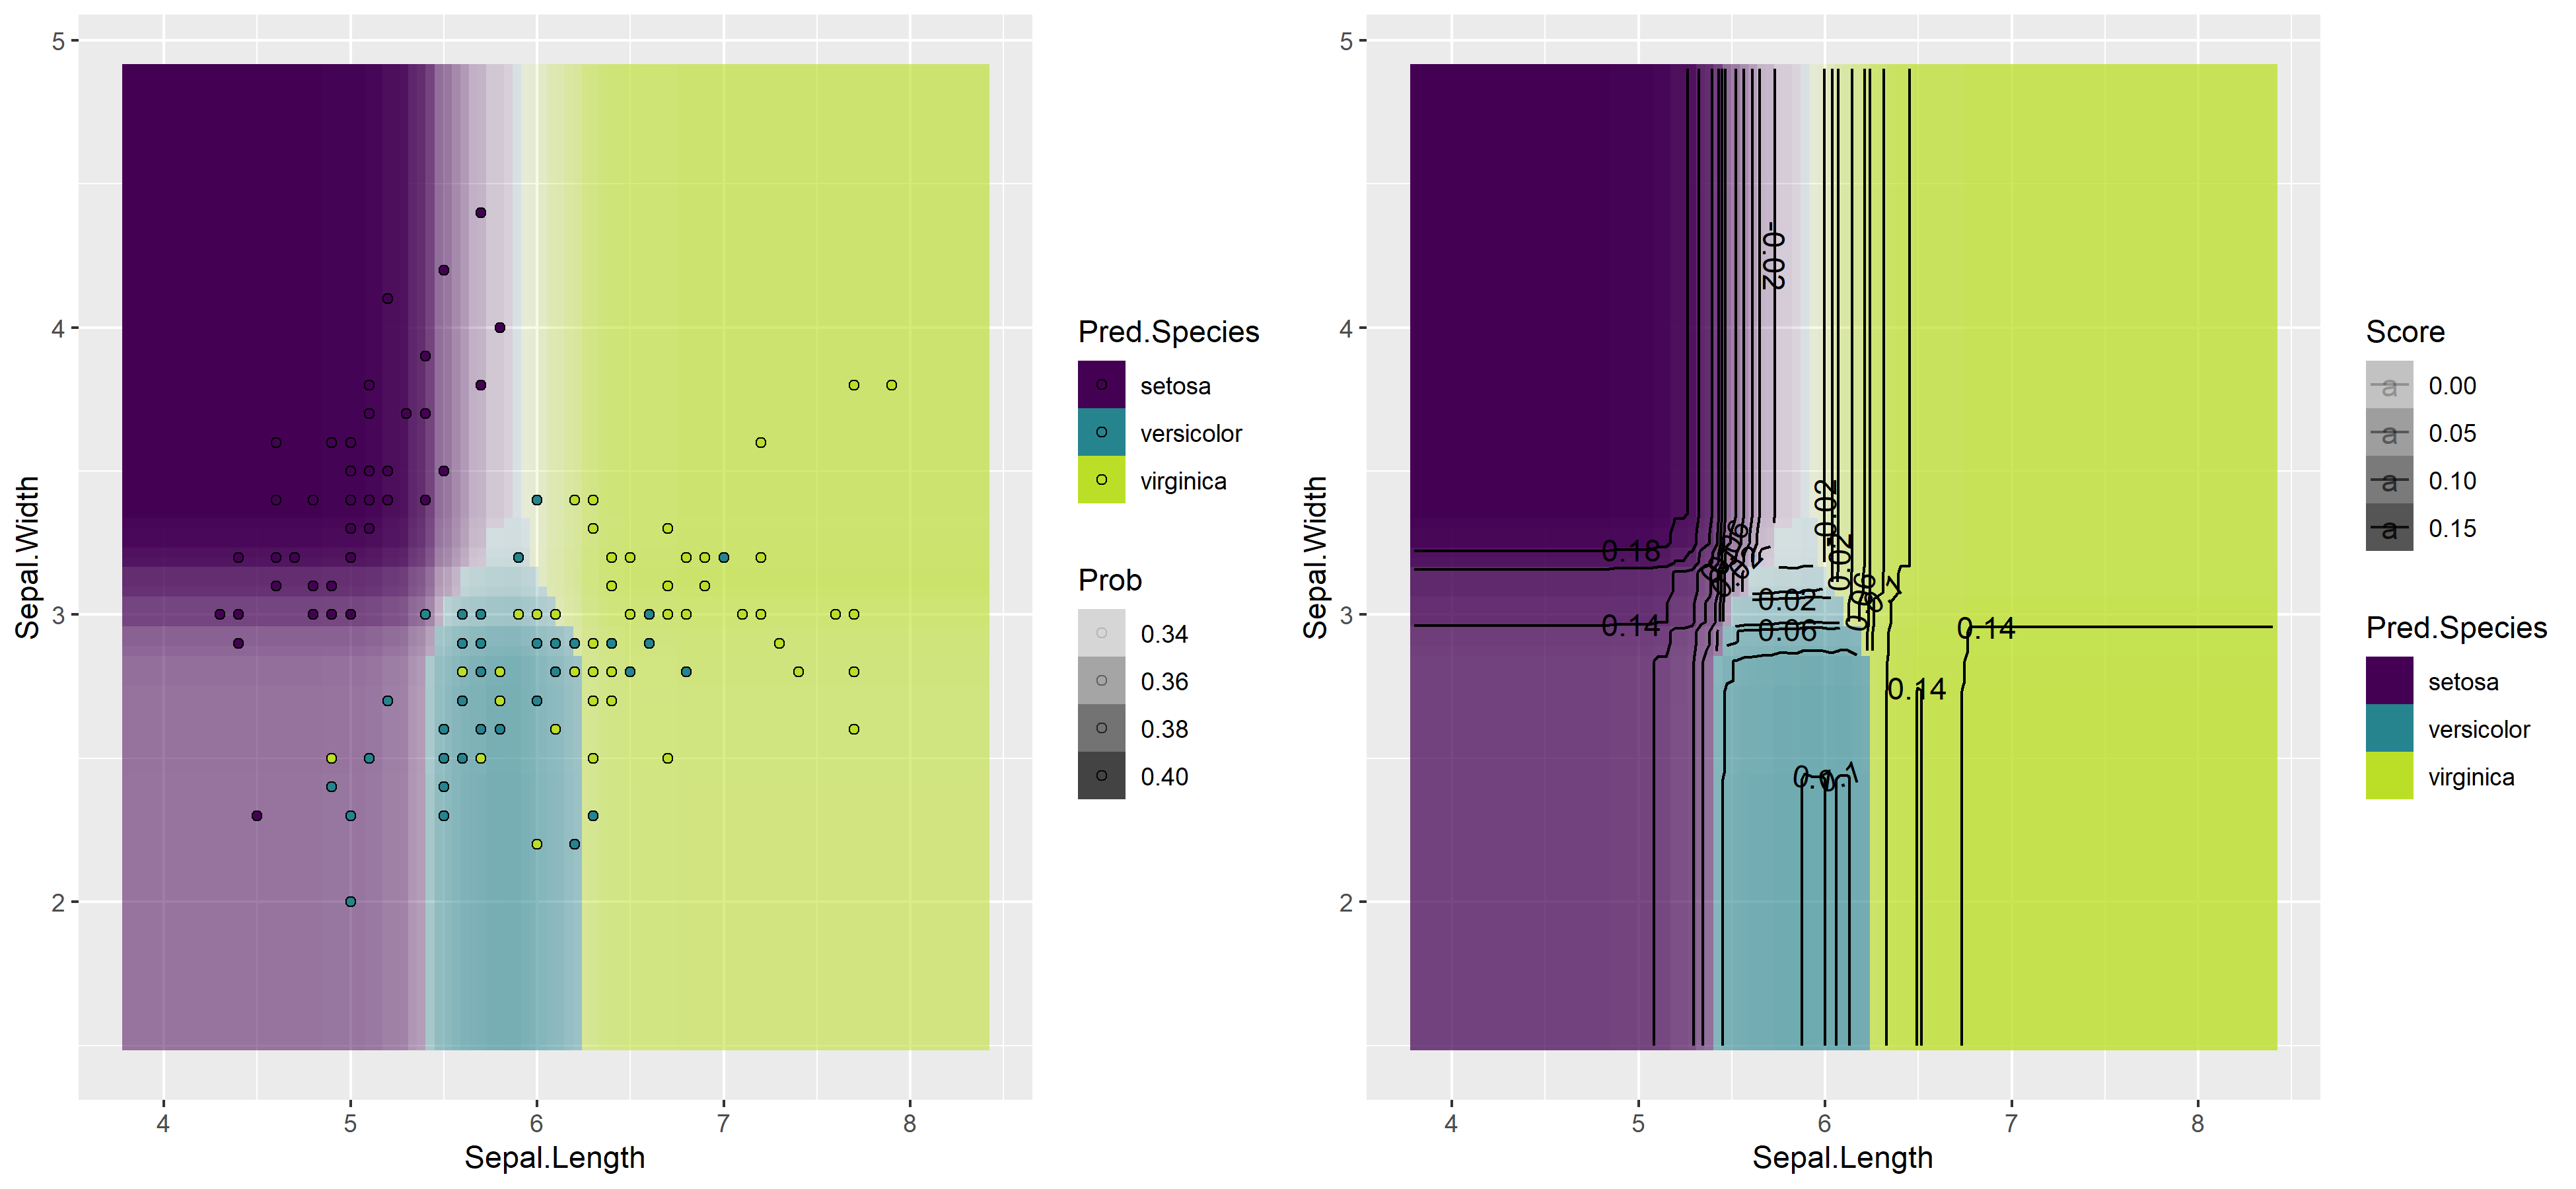
\includegraphics[width=\textwidth]{
  ../slides/boosting/figure/boosting_multiclass_100} \\
  \tiny{Boosting prediction surface with tree base learners for \texttt{iris} 
  data after 100 iterations (\textit{right:} contour lines of discriminant 
  functions)}
\end{minipage}

\end{frame}

% ------------------------------------------------------------------------------

\begin{frame}{Gradient Boosting -- method summary}

\footnotesize

\highlight{Empirical risk}

\begin{itemize}
  \item \textbf{Outer loss} used to compute pseudo-residuals -- error of 
  current model fit \\
  $\Rightarrow$ arbitrary \textbf{differentiable} loss function
  \item \textbf{Inner loss} used to fit next base learner component to 
  current pseudo-residuals \\
  $\Rightarrow$ typically, \textbf{quadratic loss}
\end{itemize}

\medskip

\highlight{Optimization} ~~ \textbf{Functional gradient descent} for outer 
optimization loop

\medskip

\highlight{Hyperparameters}

\begin{itemize}
  \item \textbf{Ensemble size}, i.e., number of base learners
  \item \textbf{Complexity} of base learners (depending on type used)
  \item \textbf{Learning rate}, i.e., impact of next base learner
\end{itemize}

\medskip

% \highlight{Runtime behavior} ~~ $\mathcal{O}(M \cdot n \cdot p)$ 
% for $M$ base learners, $n$ observations and $p$ features

\end{frame}

% ------------------------------------------------------------------------------

\begin{frame}{Gradient Boosting -- Pro's \& Con's}

\footnotesize

\begin{columns}[onlytextwidth]
  \begin{column}{0.5\textwidth}
    \highlight{Advantages}
    \footnotesize
    \begin{itemize}
      \positem Powerful \textbf{off-the-shelf} method for supercharging weak 
      learners' performance
      \positem High predictive \textbf{performance} that is hard to outperform
      \positem Translation of most of \textbf{base learners'} advantages 
      % (e.g., for tree boosting: inherent 
      % variable selection, handling of missing data)
      \positem High \textbf{flexibility} (custom loss functions, many tuning 
      options) 
      % \positem Applicable to \textbf{unbalanced} data
    \end{itemize}
  \end{column}
  \begin{column}{0.5\textwidth}
    \highlight{Disadvantages}
    \footnotesize
    \begin{itemize}
      \negitem Hard to \textbf{interpret} -- black-box method
      \negitem Hard to \textbf{visualize}
      \negitem Prone to \textbf{overfitting}
      \negitem Sensitive to \textbf{outliers}
      \negitem Hard to \textbf{tune} (high sensitivity to variations in 
      hyperparameter values)
      \negitem Rather \textbf{slow} in training
      \negitem Hard to \textbf{parallelize}
    \end{itemize}
  \end{column}
\end{columns}

\vfill

\small

\conclbox{High-performing and flexible predictor, but rather delicate to handle}

\end{frame}

% ------------------------------------------------------------------------------

\begin{frame}{Gradient Boosting -- Practical hints}

\footnotesize

\highlight{XGBoost (extreme gradient boosting)} 

\begin{itemize}
  \item Fast, efficient implementation of gradient-boosted decision trees
  \item \textbf{State of the art} for many machine learning problems
\end{itemize}

\medskip

\highlight{Stochastic gradient boosting (SGB)} ~~ Faster, approximate version of 
GB that performs each iteration only on \textbf{random data subset} 

\medskip

\highlight{Tuning} ~~ \textcolor{blue}{Tipps??}

\medskip

\highlight{Implementation}

\begin{itemize}
  \item \textbf{R:} \texttt{mlr3} learners \texttt{LearnerClassifXgboost} / 
  \texttt{LearnerRegrXgboost}, calling \texttt{xgboost::xgb.train()}
  \item \textbf{Python:} \texttt{GradientBoostingClassifier} / 
  \texttt{GradientBoostingRegressor} from package \texttt{scikit-learn}, 
  \texttt{XGBClassifier} / \texttt{XGBRegressor} from package \texttt{xgboost}
\end{itemize}

\end{frame}